%& -job-name=report
\documentclass[leqno,a4paper]{article}
\usepackage{hyperref}
\usepackage{caption}
\usepackage[T1]{fontenc}
\usepackage[utf8]{inputenc}
\usepackage{lmodern}
\usepackage[english]{babel}
\linespread{1.25} %easier reading/grading.
\usepackage{amsmath} %d'oh
\usepackage{amsfonts}
\usepackage{graphicx}
\usepackage{bold-extra} %for \mb
\usepackage[margin=2.5cm]{geometry} %for custom margins
\usepackage{enumerate} %for special counters
\usepackage{titlesec} %for section numbering
\usepackage{ifthen}
\renewcommand\thesubsection{\alph{subsection}}
\titleformat{\section}{\it \bf \large}{{\normalfont  \bf \thesection.}}{4pt}{}[]
\titleformat{\subsection}{\it \bf \large}{{\normalfont \bf \quad \large  \thesection \thesubsection)}}{5pt}{}[]
\titleformat{\subsubsection}{\bf \it}{\qquad}{5pt}{}[]

\numberwithin{equation}{section}
\newcommand\norm[1]{\left\lVert#1\right\rVert} %http://tex.stackexchange.com/questions/107186/how-to-write-norm-which-adjusts-its-size
\renewcommand{\O}{\mathcal{O}}
\renewcommand{\bf}{\bfseries}
\renewcommand{\sc}{\scshape}
\renewcommand{\it}{\itshape}
\renewcommand{\div}{\text{div }}
\renewcommand{\Re}{\mathbb{R}}
\newcommand{\op}{\left(}
\newcommand{\cp}{\right)}
\newcommand{\N}{\mathbb{N}}
\newcommand{\mb}{\mathbf}
\newcommand{\nn}{\\\nonumber}
\newcommand{\curl}{\text{curl }}
\newcommand{\inp}[2]{\left<#1, #2\right>}
\renewcommand{\d}[1]{\,\text{d}#1}
\newcommand{\pdrv}[2][x]{\frac{\partial #2}{\partial #1}}
\newcommand{\drv}[2][x]{\frac{\text{d} #2}{\text{d} #1}}
\renewcommand{\maketitle}[2][]{\begin{center}
{{\bf \huge \sc #2\\
\ifthenelse{\equal{#1}{}}{}{{\vspace{-12pt} \Large #1}\\\vspace{5pt}}
\begin{minipage}{0.4\textwidth}
  \raggedright
  {\large
   Roel Deckers}\\
   \normalsize
   roel@codingcat.nl\\
   930830-T150
\end{minipage}
\hfill
\begin{minipage}{0.4\textwidth}
  \raggedleft
  \large
  Caryl Zarate\\
  \normalsize
  caryl.zarate@gmail.com\\
  890130-4207
\end{minipage}
}}
\vspace{-1. cm}\rule[2.5 cm]{16 cm}{1 pt}
\vspace{-2.0 cm}
\end{center}}

\usepackage{algorithm}
\usepackage[noend]{algpseudocode}
\graphicspath{./plots}
\begin{document}
  \maketitle[Programming of Parallel Computers]{Project Ising Model}
\begin{abstract}
    The Ising model is a statisticall model for ferromagnetism. A popular algorithm for simulating this model is the so called Metropolis algorithm.
    Useful results require many iterations however, and therefore performance should be considered when implementing the Metropolis algorithm. In this report
    a  GPGPU implementation using OpenCL is presented and discussed.
\end{abstract}

\section{Introduction}
\subsection{The Ising Model}
The Ising model is a statistical model for ferromagnetism. It concerns the magnetic dipole moments of atomic spins, in the model these spins can be
in one of two states, spin-up (+1) or spin-down (-1). Usually these spin elements are laid on an equidistant grid with a periodic boundary condition. This model can be used to determine several interesting properties
of ferromagnets, such as phase-transitions, total-energy, total magnetism and heat capacity in vacuo or the presence of an external magnetic field.
\par In this report we focus on equidistant grids in two dimensions of varying sizes. As our focus is on optimizing the performance of the algorithm and not the underlying
physics we will only present the gradient of the energy with respect to the binding strength in between spin-sites in vacuo as a proof-of-correctness.

\subsection{Metropolis Algorithm}
A step of the Metropolis algorithm works as described in algorithm \ref{alg:metro}, this step is repeated several times in order to reach an equilibrium state.
It should be noted that there are a variety of ways to pick which spin-site to check. This can be done by selecting a random site, or by walking over each point sequentially as well as using red-black coloring.
We will employ the latter technique and defer any discussion on the statisticall properties of these various sampling methods as these would go beyond the scope of this report.
\begin{algorithm}
  \caption{Metropolis Algorithm step in Two Dimensions}\label{alg:metro}
  \begin{algorithmic}[1]
    \State $\textit{Coords} \gets \text{An appropriately chosen spin-site.}$\Comment{Spin sites can be selected in various ways.}
    \State $\textit{C} \gets \text{Spin value at }Coords$
    \State $\textit{N} \gets \text{Spin value at }Coords + (0, +1)$
    \State $\textit{E} \gets \text{Spin value at }Coords + (+1, 0)$
    \State $\textit{S} \gets \text{Spin value at }Coords + (0, -1)$
    \State $\textit{W} \gets \text{Spin value at }Coords + (-1, 0)$
    \State $\textit{f} \gets N+E+S+W$
    \State $\textit{r} \gets \text{A random number from the uniform distribution } \left[0,1\right]$
    \If {$r \leq \exp(-2C(Jf+B))$}\Comment{$J$ is the binding constant, $B$ the external magnetic field.}
      \State $\text{Flip the value at }Coords.$
    \EndIf
  \end{algorithmic}
\end{algorithm}


\section{Implementation}
When updating the Ising Model using the Metropolis algorithm and a red-black updating scheme one can update half of the points in parallel at each step.
This highly parallel scheme lends itself well to be adopted to massively parallel accelerators such as GPU (For this report we have targeted a AMD r280x).
Although the algorithm has a relatively high memory-access to computation ratio steps can be taken to reduce this ratio. A difficulty when implementing the Metropolis
algorithm in OpenCL is the fact that OpenCL does not have a build in random number generation function and thus one has to implement their own. And because many random number generators
require the user to keep track of a state, and we need a large amount of independent generators for all the sites this adds a great deal of overhead. Luckilly a simple linear congruential generator of the form
$x \gets x * \texttt{0xDEECE66D} + \texttt{0xB} \mod 2^{32}$ seems to be adequate and using some tricks we will discuss later, we have managed to reduce the memory requirement for the states to half a bit per spin-site.
\par We will now quickly describe the various implementations we will show in this report.

\subsection{Naive-transfer}
  This is a straigthforward implementation of the Metropolis Algorithm using red-black coloring and for each iteration (updating all red or black points) random numbers are generated on the host and transferred asynchronouslly to the device.
  This implementation serves as a baseline worst-case performance.
\subsection{Naive-rng}
  This implementation is non-optimized but generates the random numbers on the device using the previously discussed LCG.
\subsection{Optimized}
  This is the fully optimized implementation. The applies optimizations are
  \begin{enumerate}
    \item{{\em Cached flip chances: }Looking at algorithm \ref{alg:metro} we note that $f$ can only ever take 10 distinc values at most, and it is therefore possible to cache these values in a lookup table instead of evaluating the expensive exponential function.
    We do so by generating the table on the host and then storing it in the fast (and cached) constant memory.}
    \item{{\em Double red-black coloring:} use a double red-black coloring scheme. First the total grid is dividided into blocks of $128\times128$ sites and colored red-black. Each block is then updated using another red-black scheme.
    This speeds up the simulation by allowing us to reduce the loads from global memory by first caching a block into the much faster local memory. It has been suggested by others that it is possible to perform several updates on the cached block before moving on to the
    next block iteration, we have implemented this and the amount of "inner loops" can be controlled by the parameter $k$. It seems however that doing so leads to incorrect results.\footnote{This might be a misreading of the paper I used as a reference, as it was a single line without any other context or code, or due to
    a different random number generator, as the quality of the results is somewhat dependent upon the quality of the random numbers.}}
    \item{{\em Reduced data-load by storing spins in a single bit: } Because spins can only be up or down, it is theoretically (and practically) possible to store them in a single bit each. We have done so by organizing the data in a layout
    where the first 32 bits correspond to the first 32 red spin-sites, followed by the first 32 black spin-sites and then it repeats. Proccessing this data requires a bit more work of course. For example when calculating $f$ we need at least 4 bits per site to generate an index.
    For a full description of how we have solved this we reffer to the source code\footnote{It's a little big magic-y, but also very hard to explain in text.}
    }
    \item{{\em Reduced data load by reusing the rng:} This optimization is the kind which could break the actual results, but luckilly it works for us, as it is based on trying to get the lowest quality random numbers we can get away it.
    Now LCGs are already highly correlated and low-quality random numbers. What we ended up doing is keeping one (32 bit) state per work item, which updates 64 sites, leading to a half-a-bit per site. We try to reduce the correlation by creating 4 streams by XOR-ing the state which randomly chosen constants and then looping over using each of these streams
    and writting back the non XOR-ed result to the state when we are done.}
  \end{enumerate}
  All of these optimizations do come at the price of a minimum size of $256\times256$, which is relatively large. Even larger systems could be optimized more by using larger block sizes as each block needs all the border points in addition to its interior points and
  due to the bit-packing we have used these borders are a significant part of the total memory loads. (roughly 1/3).

\section{Results}
The result of our work can be summarized in two graphs, figure \ref{fig:perf} which show the performance increase of our methods, and figure \ref{fig:E} which shows the consistency of our method.
Note how the results for $k > 1$ are inconsistent with the others. This might be an issue of convergence (the system has trouble reaching equilibrium with the reduced loop count) or due to a subltelty with the PRNG.
\par In terms of performance we see a clear increase by using our optimized method, save for one point at a system size of $2^8$ which seems to be due to the reduced number of work-items not saturating the device. Using $k > 1$ does give a significant speed-up still
however significantly less than what we gained in previous steps.

\begin{figure}[!Hhp]
  \cenetring
  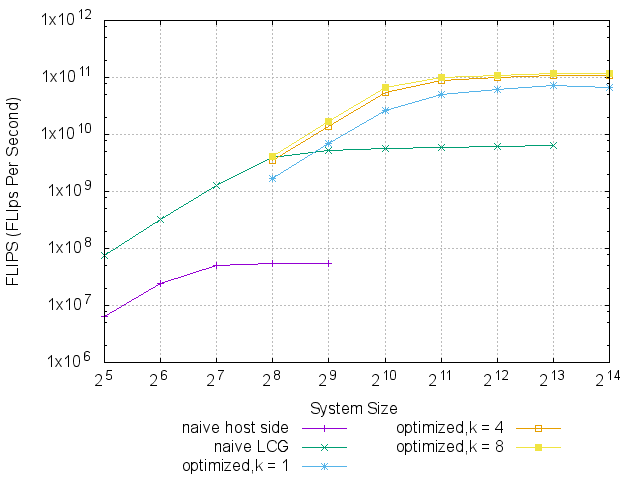
\includegraphics[width=\textwidth]{plots/timing.png}
  \label{fig:perf}
  \caption{Performance of various methods as a function of system size}
\end{figure}

\begin{figure}[!Hhp]
  \cenetring
  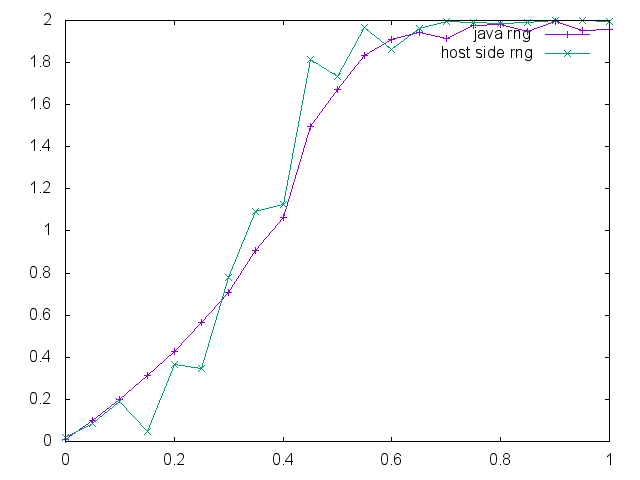
\includegraphics[width=\textwidth]{plots/MvJ.png}
  \label{fig:E}
  \caption{Gradient of the energy for the various methods.}
\end{figure}

\section{Conclusion}
We can conclude that we have successfully optimized our Ising model implementation, and demonstrated the importance of both reducing transfers between host and device and from memory to compute-unit. We applied a novel bit-packing method to increase the ratio of computation to memory access and
greatly reduced the memory requirements for both the spin-states as well as the PRNG. Further improvements could perhaps be made by increasing the block size and/or improving the data layout to improve data-traffic for the dual-red-black coloring scheme.
\begin{appendices}
  \section{A note on measuring performance.}
  It is common to measure the performance of Ising Models using either flips-per-second or time-per-flip and hence this was used in this report. However, for practicall purposes we want sample $N$ independent states at a certain equilibrium (due to the stochastic nature these will vary, and in fact
  the variance is of physicall importance) and therefore what we should be measuring is the real-time autocorrelation time of the system. The autocorrelation time is a measure of how long it takes for a state to become independent of its initial configuration. Using a stronger PRNG for example might
  lead to a much lower autocorrelation time (in terms of iterations) at the cost of a much longer iteration time.
\end{appendices}


\end{document}
